\section{Restart strategies}

\frame{\tableofcontents[currentsection]}

\begin{frame}
    \frametitle{What should a child specification contain?}
    \begin{itemize}
        \item Child specs aren't enough
        \item What if processes depend on each other?
    \end{itemize}
\end{frame}

\begin{frame}
    \frametitle{Different restart strategies}
    \begin{itemize}
        \item One for one
        \item One for all
        \item Rest for one
    \end{itemize}
\end{frame}

\begin{frame}
    \frametitle{One for one}
    \begin{center}
        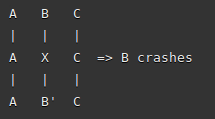
\includegraphics{05_one_for_one.png}
    \end{center}
\end{frame}

\begin{frame}
    \frametitle{One for all}
    \begin{center}
        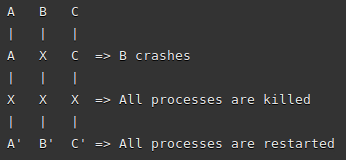
\includegraphics[scale=0.7]{05_one_for_all.png}
    \end{center}
\end{frame}

\begin{frame}
    \frametitle{Rest for one}
    \begin{center}
        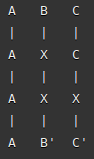
\includegraphics{05_rest_for_one.png}
    \end{center}
\end{frame}

